\section{Entanglement generation}\label{sec:4:entanglement-generation}
If the state $\rho$ is reconstructed using repeated measurements, but the initial placement of the particles were slightly different for each measurement, this is effectively comparable to an averaging process over all variations of the initial parameters in the setup.
As mentioned above, this averaging results in a mixed state and for large variations $\Delta \theta$ and $\Delta L$ this process can destroy entanglement.
To see this, I calculate the effective measured state $\mean{\rho}$ using
\begin{equation}\label{eq:4:average-density}
  \mean{\rho} = \int_{-\infty}^{\infty} \dd \theta_A p(\theta_A) \int_{-\infty}^{\infty} \dd \theta_B p(\theta_B) \int_{-\infty}^{\infty} \dd L_A p(L_A) \int_{-\infty}^{\infty} \dd L_B p(L_B) \ \rho(\theta_A, \theta_B, L_A, L_B)
\end{equation} 
where $p(\,\cdot\,)$ is the gaussian probability distribution. Both $\theta$ and $L$ are distributed normally with mean $0$ and standard deviation $\Delta \theta$ or $\Delta L$ respectively. $\rho(\theta_A, \theta_B, L_A, L_B)$ is the state of a single measurement, dependent on the initial parameters $\theta_{A(B)}$ and $L_{A(B)}$ of the setup.
The initial state $\rho_0$ at $t=0$ is given similarly as before by eq. \eqref{eq:2:initial-state} at the beginning of \cref{cha:first-look}.
During the time evolution, not only the mutual gravitational interaction between the particles must be taken into account, but also the dephasing due to the Casimir interaction between the particles and the Faraday shield.
A single superposition state $\ket{\psi^i_{A(B)}}$ ($i = 1, 2$) accumulates the phase $\phi^i_{A(B),\,\mathrm{Cas}}(t)$ during time evolution due to the casimir interaction where the phases are given by
\begin{equation}
  \phi^i_{A(B),\,\mathrm{Cas}}(t) = \frac{t}{\hbar}
  \begin{cases}
     \frac{3 \hbar c}{8 \pi} \left(\frac{\varepsilon_r - 1}{\varepsilon_r + 2}\right) \frac{R^3}{(L^i_{A(B)})^4} & \text{for large separations (LSL)} \\
    \frac{\hbar c \pi^3}{720} \varphi(\varepsilon_r) \left(\frac{\varepsilon_r - 1}{\varepsilon_r + 1}\right) \frac{R}{(\mathscr{L}^i_{A(B)})^2} & \text{for small separations (PFA)}
  \end{cases}
\end{equation}
Here, both analytical limits of the Casimir interaction discussed in \cref{cha:casimir-effect} have been used.
The particle-shield separations $L^i_{A(B)}$ and $\mathscr{L}^i_{A(B)} = L^i_{A(B)}-R$ are dependent on the initial (varying) positions of each particle.
In full generality, they are given by
\begin{equation}\label{eq:4:L-casimir}
  L^i_{A(B)} = L + L_{A(B)} - \frac{d}{2} \pm \frac{\Delta x_{A(B)}}{2} \sin(\delta + \theta_{A(B)})
\end{equation}
where $\pm$ distinct between $i=1$ and $i=2$ and $\delta = \alpha, \beta$ was used as an abbreviation.
The mutual gravitational interaction of the state $\ket{\psi^i_A}\otimes\ket{\psi^j_B}$ is given similar to before by the accumulated phase
\begin{equation}
  \phi^{ij}_\mathrm{Grav}(t) = \frac{t}{\hbar} \frac{G M_A M_B}{L^{ij}} .
\end{equation}
The separation distance $L^{ij}$ between the states $A_i$ and $B_j$ in full generality is given by
\begin{multline}\label{eq:4:L-gravity}
  L^{ij} = \sqrt{\left(2L + L_A + L_B \pm \frac{\Delta x_A}{2}\sin(\alpha + \theta_A) \mp \frac{\Delta x_B}{2}\sin(\beta + \theta_B)\right)^2 +} \\ \overline{\left(\frac{\Delta x_A}{2}\cos(\alpha + \theta_A) \pm \frac{\Delta x_B}{2}\cos(\beta + \theta_B)\right)^2} .
\end{multline}
Expanding the accumulated gravitational- and Casimir phases to first order in $\Delta x_{A(B)} \ll L$, $\theta_{A(B)} \ll 1$ and $L_{A(B)} \ll 1$ (which is possible since all these variations are very small, as seen later), the averaging of the evolved state $\mean{\rho}$ eq. \eqref{eq:4:average-density} can be performed analytically (for an exemplary calculation see \cref{apx:average-density}).
It turns out that with $\Delta \theta_A = \Delta \theta_B \equiv \Delta\theta$ and $\Delta L_A = \Delta L_B \equiv \Delta L$ all off-diagonal elements of the averaged state $\mean{\rho}$ (the so-called \emph{coherences}) are given in the form
\begin{equation}\label{eq:4:average-density-element}
  \mean{\rho_{kl}} = \frac{1}{4} e^{i \Delta \phi_{kl}(t)} \exp{-\frac{(\xi_{kl})^2}{2} (\Delta\theta)^2 t^2} \exp{-\frac{(\zeta_{kl})^2}{2} (\Delta L)^2 t^2}
\end{equation}
where $\Delta \phi$, $\xi$ and $\zeta$ are substitutes for rather lengthy expressions that depend on the particle-shield separation $L$, the orientation of the cat-state $\alpha, \beta$, the masses of the particles $M_{A(B)}$ and the superposition size $\Delta x_{A(B)}$.
It becomes evident that for large times $t\rightarrow \infty$ or for large variations in the placement $\Delta \theta, \Delta L \rightarrow \infty$ these off-diagonal elements tend to zero which leads to a continuous and monotonic loss of purity, resulting in the maximally mixed state $\tr\rho^2 = 1/4$ - which obviously is not entangled.
% \begin{theorem}
%   Let $\rho$ be an $N\times N$ density matrix with $\rho_{ii} = 1/N$ and $\rho_{ij} = f_{ij}(t)$ ($i\neq j$) with an arbitrary functions $f\in C^1(\mathbb{R}^+\rightarrow\mathbb{C})$ with properties $\lim_{t\rightarrow\infty}f(t)=0$ and $\Re{f}$ decreasing. Then the purity $\pur{\rho}$ is continuously decreasing.
% \end{theorem}
% \begin{proof}
%   The purity is given by
%   \begin{equation}
%     \pur(\rho) = \tr\rho^2 = \sum_{i=1}^{N}\rho_{ii}^2 + \sum_{i \neq j}\abs{\rho_{ij}}^2 = 1/N + \sum_{i \neq j}\abs{f_{ij}(t)}^2
%   \end{equation}
%   The time evolution of the purity is given by
%   \begin{equation}
%     \dv{t}\pur(\rho) = \sum_{j\neq j} 2 f_{ij}(t)\dv{f_{ij}(t)}{t} \leq 0
%   \end{equation}
%   which 
% \end{proof}
For large variations in the placement of the particles, one therefore expects the loss of coherence and thus of entanglement.

The resulting logarithmic negativity of the averaged state $E_N(\mean{\rho})$ was computed numerically for different values of $\Delta \theta$ and $\Delta L$ and is shown in \cref{fig:4:EN-delta-theta}.
\begin{figure}[!htb]
  \centering
  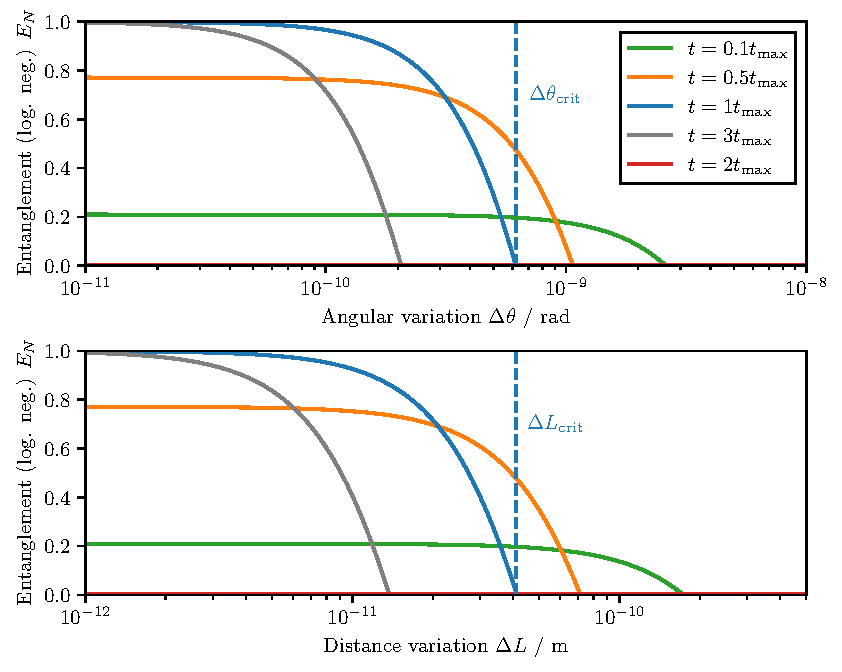
\includegraphics[width=\textwidth]{./../figures/theta-variance/EN-deltaTheta-deltaL.pdf}
  \caption{Entanglement quantified by the logarithmic negativity (eq. \eqref{eq:2:logarithmic-negativity}) dependent on the angular variation $\Delta\theta$ and the distance variation $\Delta L$ in the parallel configuration. The entanglement is shown at different times, where $t_\mathrm{max} \approx 258\si{ms}$ is the time of maximal entanglement from eq. \eqref{eq:2:t-max-parallel}. At the critical point $\Delta \theta_\mathrm{crit}$ or $\Delta L_\mathrm{crit}$ all entanglement is lost.}
  \label{fig:4:EN-delta-theta}
\end{figure}
For this figure, the parallel orientation $\alpha = \beta = 0$ was used at times relative to the time of maximum entanglement $t_\mathrm{max}$ from eq. \eqref{eq:2:t-max-parallel}.
In this special case, the entanglement is given by
\begin{equation}\label{eq:4:log-neg-analytical}
  E_N(\mean{\rho}) = \max\left\{ 0, \log_2\left(e^{-\gamma}\left(\cosh\gamma + \abs{\sin \Delta \phi}\right)\right) \right\}
\end{equation}
where the definition of the decoherences $\gamma$ can be found in \cref{apx:average-density} and $\Delta \theta$ in the parallel orientation is given by eq. \eqref{eq:2:definition-delta-phi}.
For \cref{fig:4:EN-delta-theta} the radius of the particles was set to $R=1\times 10^{-5}\si{m}$ with corresponding mass $M_A = M_B = 4/3\, \pi R^3 \rho_\mathrm{Silica} \approx 1.1\times 10^{-11}\si{kg}$.
A particle-shield separation of $L=2R$ and a superposition size of $\Delta x_A = \Delta x_B = 100\si{nm}$ were chosen.
In the rest of the thesis, if not otherwise specified, these parameters are used as a default.
For convenance, they are displayed in \cref{tab:paramters}.
They are chosen in the specific orders of magnitude, because they result in a feasible low experiment-time $t_\mathrm{max}\approx 258\si{ms}$ and are in the region of what is soon\footnote{\q{Soon} in this context means still a long time, but the experiment could be doable within this century.} possible \cite{Aspelmeyer_2024}.
Other proposals suggest a similar parameter set generally differing only by a single magnitude (see e.g. the Tab. 1 in Ref. \cite{Rijavec_2021}).
It is important however to stress out, that all these parameters are orders of magnitude away of from what is experimentally reachable today.
The largest mass that was studied in matter-wave interferometry is in the order of $4\times 10^{-23}\si{kg}$ \cite{Fein_2019} with an superposition size of $\Delta x \gtrsim 500\si{nm}$.
For solid state mechanical systems quantum control and in particular groundstate cooling up to masses in the order of $10^{-13}\si{kg}$ \cite{OConnell_2010}, $10^{-11}\si{kg}$ \cite{Lee_2011} and $10^{-8}\si{kg}$ \cite{Bild_2023} with very short coherence times $\lesssim 1\si{\mu s}$ have been demonstrated.
On the contrary, the smallest mass with a measurable gravitational coupling is around $92 \si{mg}$ \cite{Westphal_2021}.
Levitated particles combine the best of both world with quantum control of large and heavy trapped solid objects as well as long coherence times up to the order of seconds \cite{Aspelmeyer_2024}.

The entanglement of the system shown in \cref{fig:4:EN-delta-theta} behaves as expected. At some critical point $\Delta \theta_\mathrm{crit}$ and $\Delta L_\mathrm{crit}$, the entanglement is completely lost.
This critical point is analytically can in special cases be computed analytically using eq. \eqref{eq:4:log-neg-analytical} and is given by
\begin{equation}\label{eq:4:theta-crit-analytical}
  \theta_\mathrm{crit} = \frac{\log(1 + \sqrt{2})}{\gamma} \propto \gamma^{-1} .
\end{equation}
For the used parameters and in the parallel orientation, this threshold is around $\Delta \theta_\mathrm{crit} \approx 6 \times 10^{-10} \si{rad}$ and $\Delta L_\mathrm{crit} \approx 1.4 \times 10^{-10} \si{m}$, which seems quite challenging experimentally.
However, it seems like that for smaller times $t<t_\mathrm{max}$ larger variations can be tolerated for the cost of having less total entanglement.
This again is expected. For smaller times, the gravitational force did not have enough time to fully entangle the two particles, but also the decoherences (dependent on $\propto t^2$; see eq. \eqref{eq:4:average-density-element} and \cref{apx:average-density}) did not have enough time to built up. 
It is therefore logical, that if one does not require to measure a fully entangled state and less entanglement $E_N < 1$ is also sufficient, it may be beneficial to measure at a time $t < t_\mathrm{max}$. In theory, it would be enough to measure \textit{any} entanglement $E_N > 0$ but one has to make sure that no other mechanisms such as direct or indirect entanglement trough other couplings or noise sources have smaller entanglement rates (for a discussion see \cref{cha:the-shield}). 
Measuring at a earlier point in time does not only reduce the duration of a single experimental measurement, but also increases the stability against displacement variations. This optimal time of measuring for a certain required amount of entanglement is shown in \cref{fig:4:time-delta-theta}.
\begin{figure}[!htbp]
  \centering
  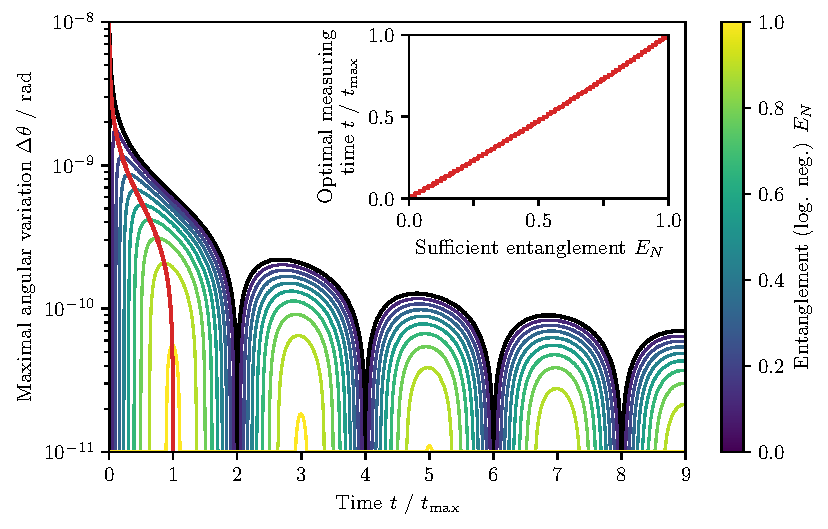
\includegraphics[width=\textwidth]{./../figures/theta-variance/time-delta-theta-crit-EN.pdf}
  \caption{Maximal angular variation for a given time and a given required amount of entanglement. The outer most black line corresponds to the time dependence of $\Delta \theta_\mathrm{crit}$. The top left as well as the red curve in the main figure shows the optimal measuring time for a sufficient amount of entanglement.
  At times $2k t_\mathrm{max}$ no entanglement can be measured.}
  \label{fig:4:time-delta-theta}
\end{figure}
The chart additionally lets one read out the corresponding maximal angular variation after a set time.
Conversely, if one is experimentally limited by a certain maximum angular variation, one can read off the corresponding best measurement time and the maximum amount of entanglement that can be obtained.
It also can be seen that at times $2k t_\mathrm{max}$, $k\in\mathbb{N}$ there is no entanglement. This corresponds to the findings from the ideal scenario in \cref{cha:first-look}. 